\documentclass[14pt]{beamer}
\usetheme{Boadilla}
\usecolortheme{whale}
\setbeamertemplate{navigation symbols}{}
\usepackage{comment}

%\setbeamertemplate{theorems}[numbered] 

\usepackage{textcomp}
\usepackage{float} 
\usepackage{multirow}
\usepackage{comment}
\usepackage{enumitem}
\usepackage{tikz}
\usepackage{algorithm}
\usepackage{adjustbox}
\usepackage{epstopdf}
\usetikzlibrary{arrows,decorations.pathreplacing,shapes}
\usepackage{amsmath}
\usepackage{multicol}
\usepackage{threeparttable}
\usepackage{mathrsfs}
\usepackage{arydshln}

%\usepackage[UTF8, heading = false, scheme = plain]{ctex}


\usepackage{amsfonts,amsthm,amssymb,amsmath}
\usepackage{graphicx,mathrsfs}
\usepackage{adjustbox}
\usepackage{multirow}
\usepackage{float} 
\usepackage{hyperref}
\usepackage{tikz}
\usetikzlibrary{backgrounds}
\usepackage{algorithm}
%\usetikzlibrary{snakes}
\usepackage{subfig}
\usepackage{ragged2e}
\usepackage{framed}
\usepackage{multicol}
\definecolor{shadecolor}{rgb}{0.9,0.9,0.9}

\setbeamerfont{frametitle}{size=\large}


% Setup appearance:


\newcommand{\labelitemi}{$\bullet$}
\newcommand{\BM}{\mathcal{B}} % Brownian motion
\newcommand{\cl}[1]{\lceil{#1}\rceil} % ceiling of a number
\newcommand{\R}{\mathbb{R}}
\newcommand{\Z}{\mathbb{Z}}
\newcommand{\cc}{\mathbb{c}}



% Author, Title, etc.

\title[Stabilization via Cost Adjustment]
{%
	\large
Inverse Optimization of Stabilizing Grand Coalitions via Cost Vector Adjustment%
}

\author[Lindong Liu] % (optional, use only with lots of authors)
%{F.~Author\inst{1} \and S.~Another\inst{2}}
{   %  \textit{Supervisor:}
  Lindong Liu
}


\date
{WHU, Dec. 10th, 2018}

\institute[] % (optional, but mostly needed)
{\footnotesize
	School of Management\\
	University of Science and Technology of China\\
    \vspace{10mm}	
	Co-authored with Xiangtong Qi (HKUST) and Zhou Xu (HKPU)
	\vspace{8mm}
}



% The main document


\begin{document}

\begin{frame}
  \titlepage
\end{frame}

%\begin{frame}{Outline}
%  \tableofcontents
%\end{frame}

\begin{frame}{Outline}
\tableofcontents
\end{frame}

\section{Preliminaries}
\begin{frame}
\centering
\large
\textcolor{blue}{\bf {\huge P}RELIMINARIES}
\end{frame}
%\subsection{Supply Chain and Cooperation}
%\subsection{Stabilizing the Cooperation}
\begin{frame}{Cooperative Game}
A cooperative game is defined by a pair $(V,C)$:
\begin{itemize}
\justifying
	\item A set $V = \big\{1,2,\ldots,v\big\}$ of players, \textbf{grand colaition};
%	\item $S = 2^V \setminus \{\emptyset\}$: set of all non-empty coalitions
	\item A \textbf{characteristic function} $C(S)$ = the minimum total cost achieved by the cooperation of members in coalition $S \in \mathbb{S}=2^V \setminus \{\emptyset\}$.
\end{itemize}

~\\The game requires:
\begin{itemize}
\justifying
	\item A cost allocation $\alpha=\big[\alpha_1,\alpha_2,\ldots,\alpha_v \big] \in \R^v$, where $\alpha_k$ = the cost allocated to each player $k\in V$.
\end{itemize}
\end{frame}


\begin{frame}{Core}
Define $\alpha(S)=\sum_{k\in S}\alpha_k$. \\~\\
A cost allocation $\alpha \in \R^v$ is in the \textbf{core} if it satisfies:
\begin{itemize}
\small
\justifying
	\item Budget Balance Constraint: $\alpha(V)=C(V)$;
	\item Coalition Stability Constraints: $\alpha(S)\leq C(S)$ for each  $S\in \mathbb{S}$.
\end{itemize}
%\pause
\vspace{-12pt}
\begin{eqnarray*}
\mathrm{Core}(V,C) = &&\bigg\{ \alpha:~ \alpha(V)=C(V), \\
&& \alpha(S) \leq C(S), ~\forall S \in \mathbb{S} \setminus \{V\},~\alpha \in \R^v   \bigg\}.
\end{eqnarray*}

\pause
\vspace{-12pt}
\textcolor{red}{However, $\mathrm{Core}(V,c)$ can be empty.}
\end{frame}


\begin{frame}{Instruments to Stabilize Grand Coalitions}
\begin{figure}[H]
\centering
\begin{minipage}[t]{0.32\textwidth}
\centering

\includegraphics[width=0.7\textwidth]{conculsion1.png}
\captionsetup{font={scriptsize}}
%\caption*{Unbalanced Game}
\end{minipage}
\begin{minipage}[t]{0.32\textwidth}
\centering
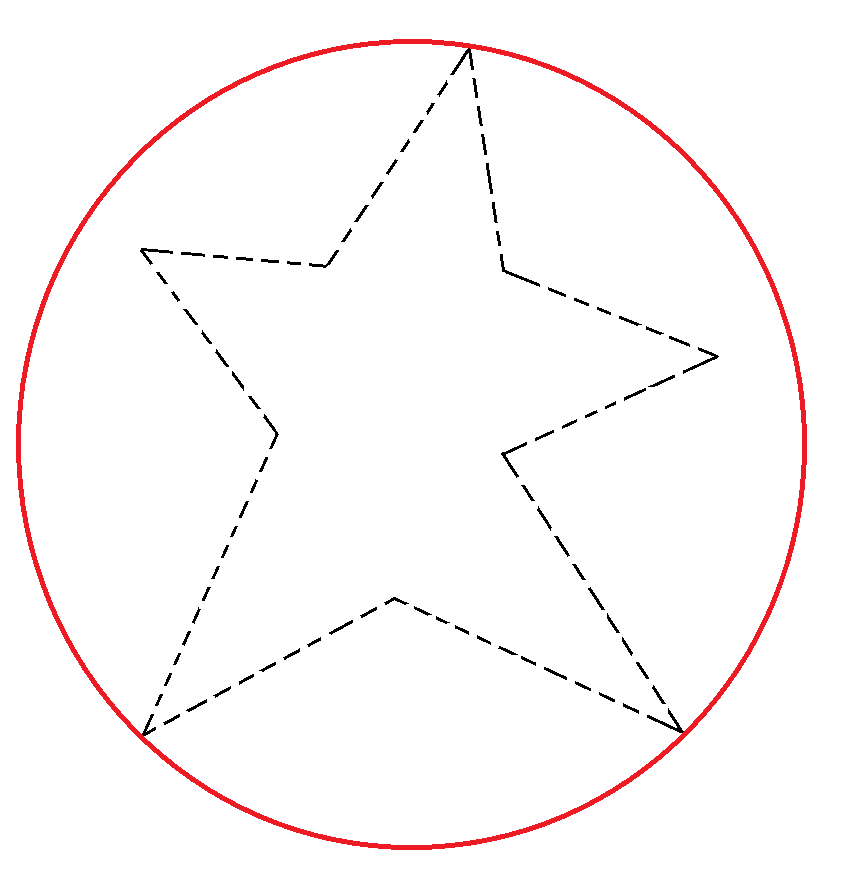
\includegraphics[width=0.82\textwidth]{conculsion3.png}
\captionsetup{font={scriptsize}}
\caption*{Filling}
\end{minipage}
\begin{minipage}[t]{0.32\textwidth}
\centering
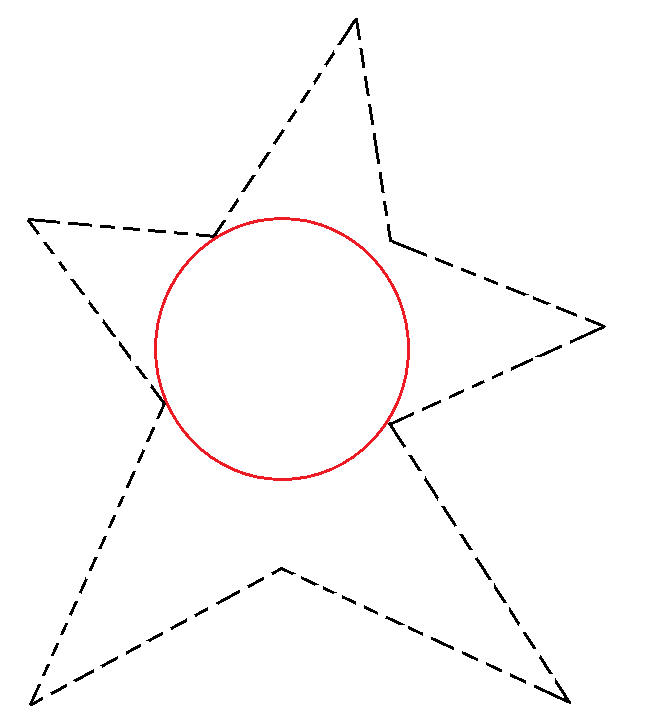
\includegraphics[width=0.7\textwidth]{conculsion2.png}
\captionsetup{font={scriptsize}}
\caption*{Cutting}
\end{minipage}
\end{figure}
\begin{figure}[H]
\centering
\begin{minipage}[t]{0.49\textwidth}
\centering
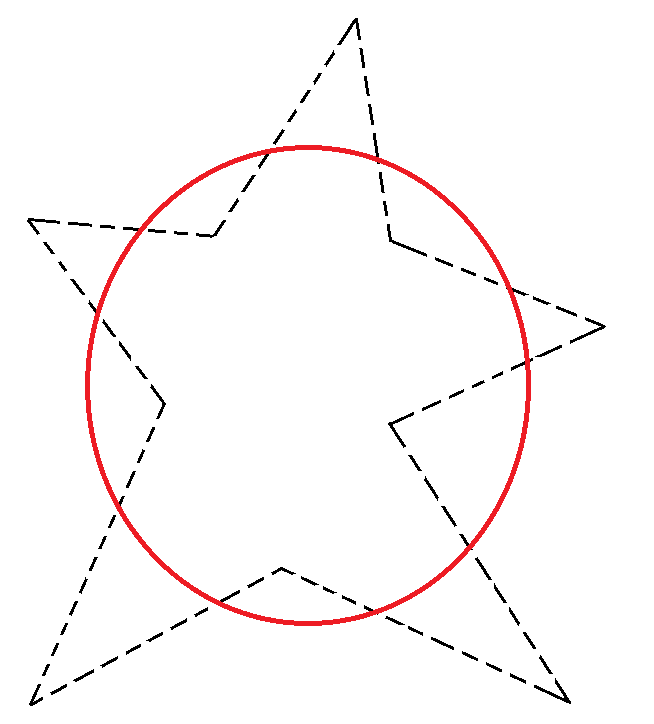
\includegraphics[width=0.42\textwidth]{conculsion4.png}
\captionsetup{font={scriptsize}}
\caption*{Simul. Filling \& Cutting}
\end{minipage}
\begin{minipage}[t]{0.49\textwidth}
\centering
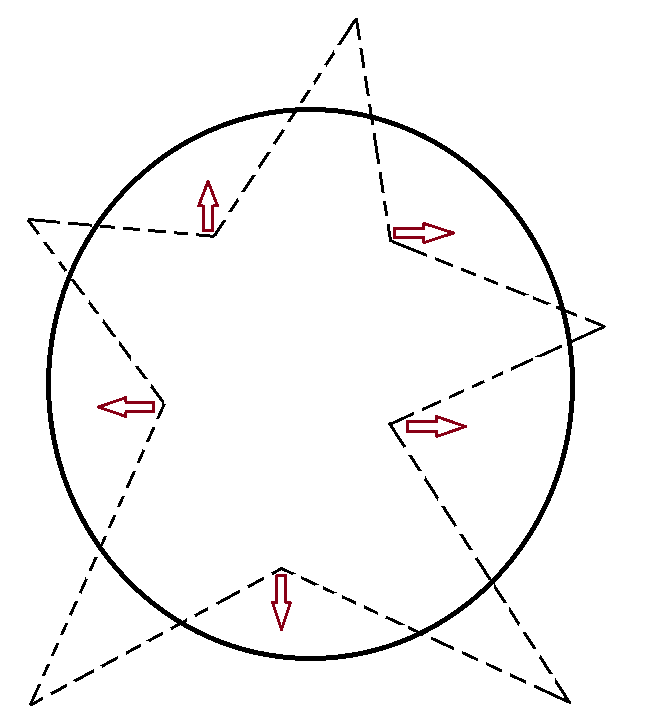
\includegraphics[width=0.42\textwidth]{conculsion5.png}
\captionsetup{font={scriptsize}}
\caption*{Stretching}
\end{minipage}
\end{figure}
\end{frame}

\begin{frame}{Existing Instruments}
\begin{small}
\vspace{-5mm}
\begin{eqnarray*}
\mathrm{Core}(V,C) = \bigg\{ \alpha:~ \alpha(V)=C(V),  ~\alpha(S) \leq C(S), ~\forall S \in \mathbb{S} \setminus \{V\}  \bigg\}
\end{eqnarray*}
\end{small}
\begin{itemize}
\small
\pause
\item Subsidization: \textcolor{red}{$\alpha(V)=C(V)-\theta$}, \textbf{$\epsilon-$core};
\pause
\item Penalization: \textcolor{red}{$\alpha(S) \leq C(S)+z$}, \textbf{least core};
\pause
\item Simul. S \& P: \textcolor{red}{$\alpha(V)=C(V)-\theta$ and $\alpha(S) \leq C(S)+z$}, \textbf{PSF}.
\end{itemize}
\pause
\vspace{-3mm}
\begin{table}[t]
	\small
	\centering
	\tabcolsep=10pt
	%\small
	\renewcommand\arraystretch{1.8}
	\vglue5pt
	\vspace{-3mm}
	\begin{tabular}[!h]{c c}
		\hline
		S.	&Caprara and Letchford (2010, MP), \textcolor{blue}{Liu et al. (2016, IJOC)}\\
		P.	&Faigle et al. (2001, IJGT), Schulz and Uhan (2010, OR)\\
		P\&S	&\textcolor{blue}{Liu et al. (2018, OR)}\\
		\hline
	\end{tabular}
	\vspace{-3mm}
	%c(V)=115
\end{table}
\end{frame}


\begin{frame}{Instruments to Stabilize Grand Coalitions}
\begin{figure}[H]
\centering
\begin{minipage}[t]{0.32\textwidth}
\centering

\includegraphics[width=0.7\textwidth]{conculsion1.png}
\captionsetup{font={scriptsize}}
\caption*{Unbalanced Game}
\end{minipage}
\begin{minipage}[t]{0.32\textwidth}
\centering
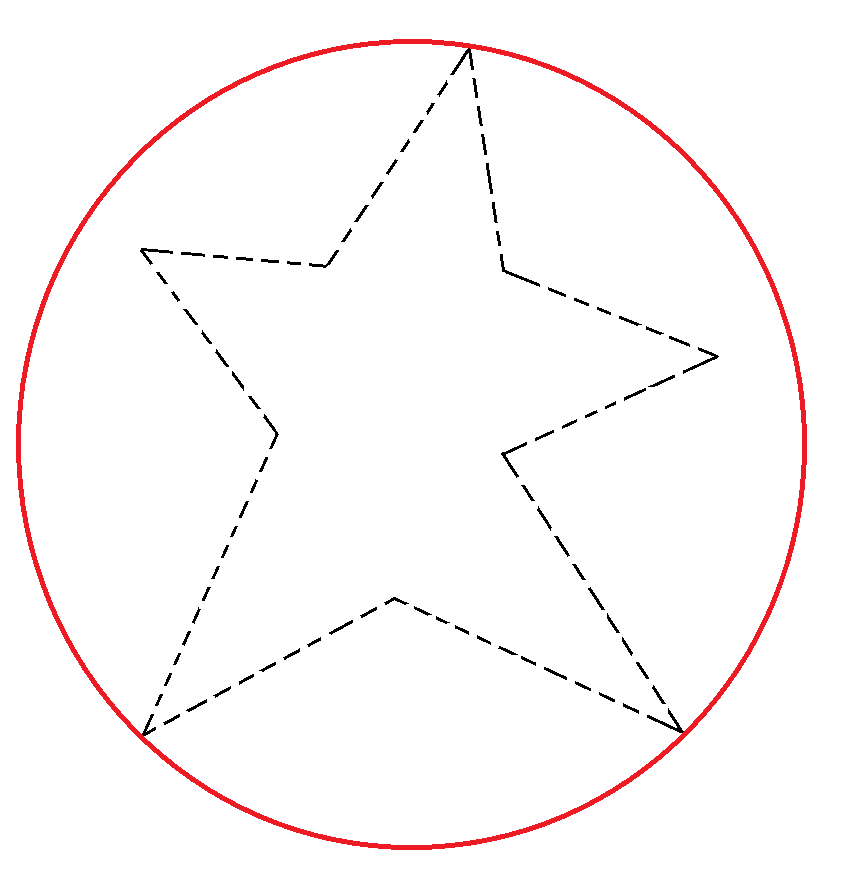
\includegraphics[width=0.82\textwidth]{conculsion3.png}
\captionsetup{font={scriptsize}}
\caption*{Subsidization}
\end{minipage}
\begin{minipage}[t]{0.32\textwidth}
\centering
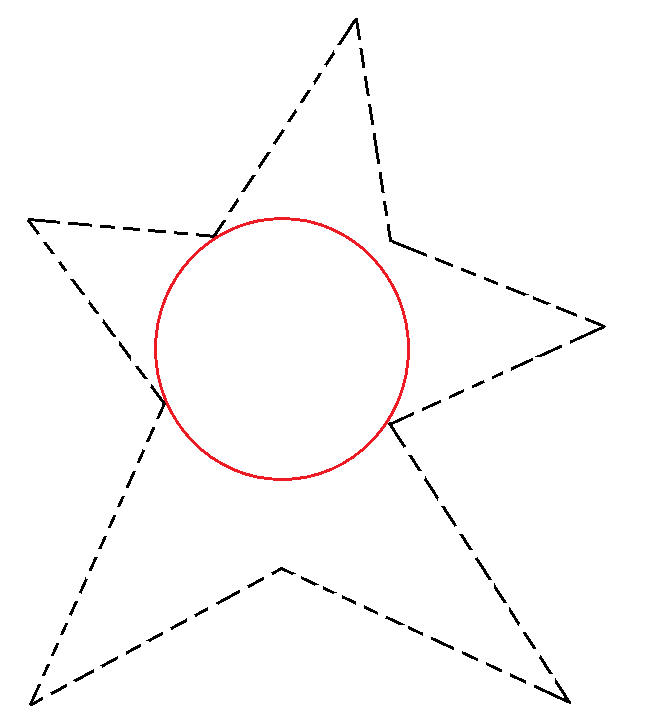
\includegraphics[width=0.7\textwidth]{conculsion2.png}
\captionsetup{font={scriptsize}}
\caption*{Penalization}
\end{minipage}
\end{figure}
\begin{figure}[H]
\centering
\begin{minipage}[t]{0.49\textwidth}
\centering
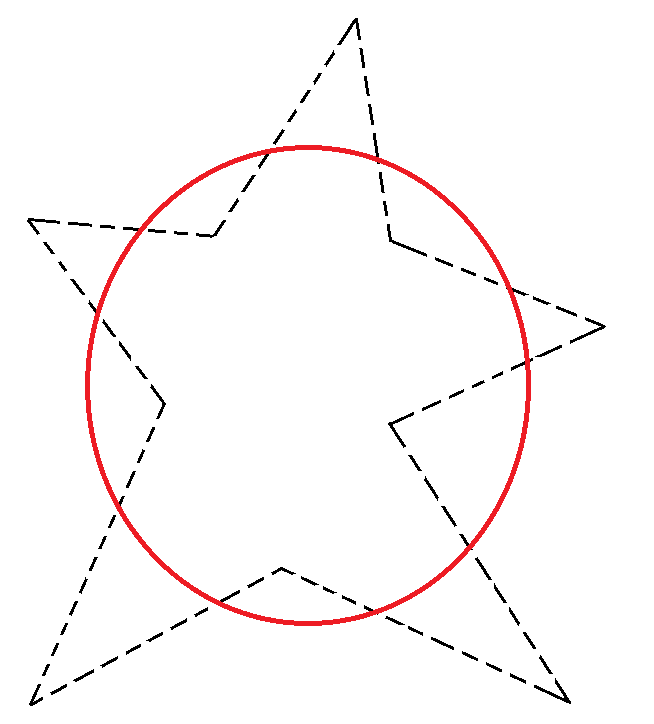
\includegraphics[width=0.42\textwidth]{conculsion4.png}
\captionsetup{font={scriptsize}}
\caption*{Simultaneously Subsidization \& Penalization}
\end{minipage}
\pause
\begin{minipage}[t]{0.49\textwidth}
\centering
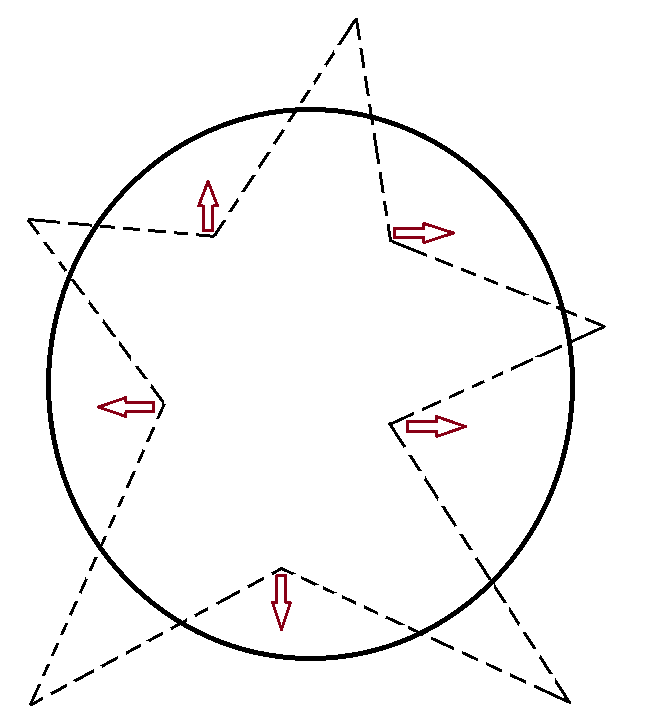
\includegraphics[width=0.42\textwidth]{conculsion5.png}
\captionsetup{font={scriptsize}}
\caption*{Cost Vector Adjustment}
\end{minipage}
\end{figure}
\end{frame}


\section{Motivation and Illustrative Example}
\begin{frame}
\centering
\large
\textcolor{blue}{\bf {\huge M}OTIVATION \& {\huge E}XAMPLE}
\end{frame}

\begin{frame}{Braess's Paradox}
\vspace{-5mm}
\begin{figure}[H]
\centering
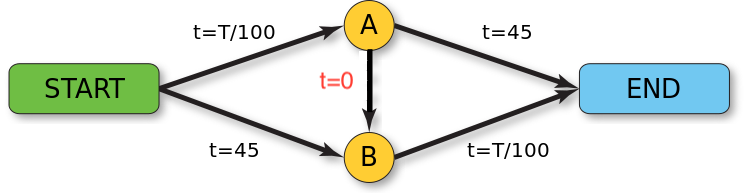
\includegraphics[width=1\textwidth]{braess.png}
\end{figure}
\centering
\vspace{-6mm}
4000 cars in total
\vspace{4mm}
\begin{columns}
\begin{column}{5.5cm}
\small
\centering
\pause
$t = 0$\\
\vspace{2mm}
$START \rightarrow A \rightarrow B \rightarrow END$\\
\vspace{2mm}
$4000/100  + 4000/100 = 80 min$
\end{column}
\begin{column}{5.5cm}
\small
\centering
\pause
$t = \infty$\\
\vspace{2mm}
$START \rightarrow A  \rightarrow END$\\
\vspace{2mm}
$START  \rightarrow B \rightarrow END$\\
\vspace{2mm}
$A=B=2000$\\
\vspace{2mm}
$2000/100+45=65min$
\end{column}
\vspace{-5mm}
\end{columns}
\vspace{-5mm}
\end{frame}



\begin{frame}{Cost Vector Adjustment on IM Games}
\justifying
\vspace{-2mm}
\begin{shaded}
$C(S)$: need to solve an optimization problem, not given.
\end{shaded}

Integer Minimization Games:
for each coalition $S \in \mathbb{S}$, an incidence vector $y^S \in \{0,1\}^{v}$, with $y_k^S=1$ if $k \in S$, and with $y_k^S=0$ otherwise, for all $k \in V$, such that
\begin{equation*}
\color{red}
C(S) = \min_{x} \{ cx: Ax \geq By^S + E, ~x \in \Z^{t} \}.
\end{equation*}
Examples: machine scheduling games, facility location games, travelling salesman games, etc.
\center
\pause
\begin{shaded}
Cost Vector Adjustment: \textcolor{red}{$ c \rightarrow d$ and $C(S) \rightarrow D(S)$}
\end{shaded}
\end{frame}



\begin{frame}{An Illustrative Example on UFL Game}
\small
\begin{columns}
\begin{column}{5.5cm}
\vspace{-10mm}
\begin{figure}[H]
\centering
\includegraphics[width=0.9\textwidth]{preliminary-example.pdf}
\end{figure}
\end{column}
\begin{column}{5.5cm}
\vspace{-5mm}
\footnotesize
\begin{shaded}
Social Optimum $C(V)$:
\begin{equation*}
10+10+3+3+2+1=29
\end{equation*}
\vspace{-5mm}
\end{shaded}
\vspace{-10mm}
\begin{shaded}
Optimal Cost Allocation Problem:
\begin{eqnarray*}
\begin{aligned}
\max ~\alpha_1 + &\alpha_2 + \alpha_3 + \alpha_4\\
s.t.~~ \alpha_1 \leq 13&,~\cdots,~\alpha_4 \leq 11,\\
\alpha_1 + \alpha_2 \leq 16,~&\cdots,~ \alpha_3+\alpha_4 \leq 17,\\
~~~~~~~~~~~~~~~&\cdots,\\
\alpha_1 + \alpha_2 + &\alpha_3 + \alpha_4 \leq 29.
\end{aligned}
\end{eqnarray*}
\vspace{-5mm}
\end{shaded}
\vspace{-10mm}
\begin{shaded}
Optimal Cost Allocation:
\begin{equation*}
7.5+6.5+8.5+4=26.5
\end{equation*}
\vspace{-5mm}
\end{shaded}
\end{column}
\end{columns}
\end{frame}

\begin{frame}{An Illustrative Example on UFL Game}
\small
\begin{columns}
\begin{column}{5cm}
\vspace{-15mm}
\begin{figure}[H]
\centering
%\caption{\label{figure:example}An example of UFL game}
\centering
\includegraphics[width=1.05\textwidth]{preliminary-example3.pdf}
\end{figure}
\end{column}
\begin{column}{6cm}
\vspace{-5mm}
\footnotesize
\begin{shaded}
\centering
Social Optimum $C(V)$: 29\\
\vspace{1mm}
Maximum Shared Cost $\alpha(V)$: 26.5
\end{shaded}
\vspace{-5mm}
\begin{shaded}
\centering
($c_{22}=1 \rightarrow 100$): \\
Optimal Cost Allocation
$$
3+11+13+2=29 ~(Stabilized)
$$
\vspace{-2mm}
\end{shaded}
\vspace{-5mm}
\begin{shaded}
\centering
($c_{14}=2 \rightarrow 100$):\\
 Optimal Cost Allocation
 $$
 8+8+7+5=28 ~(Not ~stabilized)
 $$
\vspace{-5mm}
\end{shaded}
\end{column}
\end{columns}
\end{frame}


\section{Models and Property Analyses}
\begin{frame}
\centering
\large
\textcolor{blue}{\bf {\huge M}ODELS \& {\huge A}NALYSES}
\end{frame}


\begin{frame}{Properties of an IM Game}
\vspace{-5mm}
\begin{shaded}
\centering
\small
IM Game $(V,C)$: $C(S) = \min_{x} \{ cx: Ax \geq By^S + E, ~x \in \Z^{t} \}$
\end{shaded}
\vspace{-8mm}
\begin{table}
\centering
\scriptsize
\tabcolsep=0pt
\renewcommand\arraystretch{1.9}
\begin{tabular}[!h]{c c c}
\hline
\multicolumn{1}{c}{Parameters} &\multicolumn{1}{c}{Properties}	&\multicolumn{1}{c}{Explanations}\\
\hline
\multicolumn{1}{c}{$B \geq \textbf{0}$} &\multicolumn{1}{c}{Monotonicity}	&\multicolumn{1}{c}{$C(S \cup \{k\}) \geq C(S)$ for all $S \in \mathbb{S}, ~k\in V$:$~S \cup \{k\} \in \mathbb{S}$;}\\
\multicolumn{1}{c}{$B = \textbf{0}$} &\multicolumn{1}{c}{Coalitional-Independence}	&\multicolumn{1}{c}{$C(S)$ for all $S \in \mathbb{S}$ are identical;}\\
\multirow{2}{*}{$E \geq \textbf{0}$} &\multirow{2}{*}{Subadditivity}	&\multicolumn{1}{l}{$C(S_1 \cup S_2) \leq C(S_1)+C(S_2)$ for all $S_1, S_2 \in \mathbb{S}:$}\\
&	&\multicolumn{1}{r}{$S_1 \cup S_2 \in \mathbb{S},~ S_1 \cap S_2 = \emptyset$;}\\
\hdashline
\multicolumn{1}{c}{$E = \textbf{0}$} &\multicolumn{1}{c}{Homogeneity (Assignability)}	&\multicolumn{1}{c}{$\alpha^*(V) \leq \min_x \big\{ cx:Ax \geq B\textbf{1} + E, ~x \in \R_{+}^{q} \big\}$;}\\
\multicolumn{1}{c}{$A =$\textbf{\uppercase\expandafter{\romannumeral2}},} &\multirow{2}{*}{Complete Assignability}	&\multirow{2}{*}{$\alpha^*(V)= \min_x \big\{ cx:Ax \geq B\textbf{1} + E, ~x \in \R_{+}^{q} \big\}$.}\\
\multicolumn{1}{c}{$B = \textbf{I}$, $E = \textbf{0}$} &	&\\
\hline
\end{tabular}
\end{table}
\vspace{-5mm}
\begin{tablenotes}
\tiny
\centering
 \item[1] $\alpha^*(V)=\max_{\alpha}\big\{ \alpha(V):\alpha(S) \leq C(S), ~\forall S \in \mathbb{S} \big\}$;
        ~$\textbf{0}$, $\textbf{1}$, \textbf{\uppercase\expandafter{\romannumeral2}}, $\textbf{I}$: all-zeros, all-ones, binary, identity matrices
      \end{tablenotes}
\end{frame}


\begin{frame}{GCSP via CVA Instrument}
\begin{definition}\label{definition:inverse}
\small
\justifying
Grand Coalition Stabilization Problem (GCSP) via Cost Vector Adjustment (CVA):\\
\centering \textcolor{blue}{\bf $c \rightarrow d$}, such that \textcolor{red}{\bf OCB}
\begin{itemize}
\pause
\item \textcolor{red}{Optimality:} an initial feasible solution $x^0$ is optimal to $D(V)$;
\pause
\item \textcolor{red}{Consistency:} the social optimum is consistent $C(V)=D(V)$;
\pause
\item \textcolor{red}{Balancedness:} the updated IM game $(V,D)$ is balanced.
\end{itemize}
\pause
\vspace{-3mm}
\begin{eqnarray*}\label{eqn:inverse}
~~\min_{\delta} \bigg\{f(\delta):~ d \in \mathbb{O}, ~D(V) = C(V), ~dx^0 = D(V),~\delta = d-c\bigg\},
\end{eqnarray*}
where $f(\delta) = \omega \times |\delta|$ \textcolor{purple}{($L_1$ norm)}; $\mathbb{O}$ is the Balanced Cost Vector Set.
\end{definition}
\end{frame}

\begin{frame}{GCSP via CVA $\equiv$ CIOP}
\vspace{-3mm}
\begin{shaded}
\centering
Constrained Inverse Optimization Problem (CIOP)
\end{shaded}
\vspace{-5mm}
\footnotesize
\begin{eqnarray*}
\min \bigg\{ \omega \times \big( \tau + \eta \big): d \in \mathbb{O}, ~D(V) = C(V), ~dx^0 = D(V),~\tau -\eta = d-c,\\
d \in \R^{q},~\tau \in \R^{q}_+, ~\eta \in \R^{q}_+\bigg\}.
\end{eqnarray*}
\begin{itemize}
\small
\item Only Optimality: \textcolor{red}{Inverse Optimal Solution} Problem;
\item Only Consistency: \textcolor{red}{Inverse Optimal Value} Problem;
\item Only Balancedness: \textcolor{red}{Optimal Cost Allocation} Problem.
\end{itemize}
\end{frame}


\begin{frame}{Feasibility Analyses}
\footnotesize
$$Q^{xy} = \bigg\{(x,y):~Ax \geq By+E, ~y = y(S) \text{ for some } S \in \mathbb{S}, ~x \in \mathbb{Z}^t, ~y \in \{0,1\}^v\bigg\},$$
$$\mathbb{C}^x = \text{proj}_x \bigg(\text{cone~}Q^{xy} \cap \big\{(x,y) \in \R^{q+v}: y = \textbf{1}\big\}\bigg) = \bigg\{x:~\mathbb{A}x \geq \mathbb{B}\bigg\}.$$
\begin{lemma}\label{lemma:equivalence1}
\centering
\small
EQUIVALENCE 1: The CIOP is equivalent to the following LP.
\end{lemma}
\vspace{-5mm}
\begin{small}
\begin{eqnarray*}\label{eqn:colp}
\begin{aligned}
\min ~\omega &\times \big(\tau + \eta\big)^T\\
s.t.~~dx \geq& cx^*,~\forall x \in \mathbb{C}^x,\\
d&x^0 = cx^*,\\
d-c = \tau - \eta, &\mbox{ and } d \in \R^{q}, ~\tau, ~\eta \in \R^{q}_+.
\end{aligned}
\end{eqnarray*}
\end{small}
\end{frame}


%\begin{frame}{Feasibility Analyses}
%\begin{theorem}\label{theorem:SAndN}
%\justifying
%\textbf{(Feasibility - Sufficient and Necessary Conditions)}
%For an unbalanced IM game $(V,C)$, the sufficient and necessary conditions for the feasibility of the $\mathrm{CIOP}$ is that there exists an assignable constraint 
%$$\mathbb{b} \tilde{a}x \geq \tilde{b} \mbox{ in } \big\{\mathbb{A}x \geq \mathbb{B}\big\}$$ 
%such that $cx^* \big( \tilde{a}x^0 - \tilde{b} \big)= 0,$ in addition,
%$$
%\mbox{if $cx^* > 0$, then $\tilde{b} \geq 0$; otherwise if $cx^* < 0$, then $\tilde{b} \leq 0$}.
%$$
%\end{theorem}
%\end{frame}
%
%
%\begin{frame}{Feasibility Analyses}
%\begin{theorem}\label{theorem:necessary}
%\justifying
%\textbf{(Feasibility - Necessary Conditions)}
%For an unbalanced IM game $(V,C)$, the necessary conditions for the feasibility of the $\mathrm{CIOP}$ are as follows:
%\begin{itemize}
%\item if $cx^* \neq 0$, there exists some constraint $ax \geq b\textbf{1} + e$ in $\big\{Ax \geq B\textbf{1}+E\big\}$ such that $ax^0 = b\textbf{1}+e$;
%\item if $cx^* \neq 0$, there exists some $e \geq 0$ in $\big\{E\big\}$;
%\item if $cx^* > 0$, there exists some $b\textbf{1}+e >0$ in $\big\{B\textbf{1}+E\big\}$; otherwise if $cx^* < 0$, there exists some $b\textbf{1}+e < 0$ in $\big\{B\textbf{1}+E\big\}$.
%\end{itemize}
%\end{theorem}
%\end{frame}
%
%\begin{frame}{Feasibility Analyses}
%\begin{theorem}\label{theorem:sufficient}
%\justifying
%\textbf{(Feasibility - Sufficient Conditions)}
%For an unbalanced IM game $(V,C)$, the sufficient conditions for the feasibility of the $\mathrm{CIOP}$ are as follows:
%there exists some constraint 
%$$ax \geq b\textbf{1} + e \mbox{ in } \big\{Ax \geq B\textbf{1}+E\big\}$$ such that \mbox{$ax^0 = b\textbf{1}+e$ and $e \geq 0$,} in addition,\\ if $cx^* >0$, then $b\textbf{1}+e > 0$; if $cx^* <0$, then $b\textbf{1}+e < 0$.
%\end{theorem}
%\end{frame}


\begin{frame}{Feasibility Analyses}
\begin{theorem}\label{theorem:SAndN}
\justifying
\centering
\textbf{\rm Feasibility -- Sufficient and Necessary Conditions}
\end{theorem}
\begin{theorem}\label{theorem:necessary}
\justifying
\centering
\textbf{\rm Feasibility -- Necessary Conditions}
\end{theorem}
\begin{theorem}\label{theorem:sufficient}
\justifying
\centering
\textbf{\rm Feasibility -- Sufficient Conditions}
\end{theorem}
\end{frame}


\begin{frame}{Feasibility Analyses}
\vspace{-3mm}
\begin{shaded}
\vspace{-6mm}
\centering
\small
$$C(V) = \min_{x} \{ cx: Ax \geq B\textbf{1} + E, ~x \in \Z^{t} \}$$
\vspace{-8mm}
\end{shaded}
\vspace{-3mm}
\begin{corollary}\label{corollary:sufficient}
\justifying
 Two special sufficient conditions for the feasibility of the $\mathrm{CIOP}$ are as follows: in the ILP of $C(V)$
 ~~\\
\begin{itemize}
\item[$\bullet$] there exists some \textcolor{red}{coalitional independent constraint} $ax = e$ with $e>0$ and $cx^* > 0$; or,
~~\\
\item[$\bullet$] there exists some \textcolor{red}{homogeneous constraint} $ax = b\textbf{1}$.
\end{itemize}
\end{corollary}
\end{frame}


\begin{frame}{How to Handle an Infeasible CIOP}
\vspace{-3mm}
\begin{shaded}
\centering
Motivated by the Instrument of Subsidization
\end{shaded}
\vspace{-5mm}
\footnotesize
\begin{eqnarray*}
\min \bigg\{ \omega \times \big( \tau + \eta \big): d \in \mathbb{O}(\theta), ~D(V) = C(V), ~dx^0 = D(V),~\tau -\eta = d-c,\\
d \in \R^{q},~\tau \in \R^{q}_+, ~\eta \in \R^{q}_+\bigg\}.
\end{eqnarray*}
\begin{itemize}
\small
\item[$\blacktriangleright$] $\mathbb{O}(\theta_1) \subseteq \mathbb{O}(\theta_2)$ for all $\theta_1 \leq \theta_2$;
\item[$\blacktriangleright$] $lim_{\theta \to\infty} \mathbb{O}(\theta) = \mathbb{R}^q$, the CIOP is feasible when $\theta$ is large;
\item[$\blacktriangleright$] \textcolor{red}{balancedness $\iff$ $\theta^* \leq 0$ ($f(\delta)=0$ for all $\theta \geq \theta^*$).}
\end{itemize}
\small
\centering
The CIOP is NP-hard in general
\end{frame}

\begin{frame}{How to Handle an Infeasible CIOP}
\vspace{-8mm}
\begin{shaded}
\centering
Motivated by the Instrument of Penalization
\end{shaded}
\vspace{-10mm}
\footnotesize
$$
\hat{C}(S) = \min_{x,\sigma} \bigg\{ cx + 0 \times \sigma:Ax \geq By(S) + E, ~\sigma \geq 1 - |S|/|V|, ~\sigma \in \Z_{+},~x \in \Z_{+}^{q} \bigg\}
$$
\vspace{-5mm}
\begin{eqnarray*}
\min \bigg\{ \hat{\omega} \times \big( \hat{\tau} + \hat{\eta} \big): \hat{d} \in \hat{\mathbb{O}}(\theta), ~\hat{D}(V) = \hat{C}(V), ~\hat{d}x^0 = \hat{D}(V),~\hat{\tau} -\hat{\eta} = \hat{d}-\hat{c},\\
\hat{d} \in \R^{q},~\hat{\tau} \in \R^{q}_+, ~\hat{\eta} \in \R^{q}_+\bigg\}.
\end{eqnarray*}
\vspace{-5mm}
\begin{itemize}
\small
\item[$\blacktriangleright$] the resulting CIOP is feasible;
\item[$\blacktriangleright$] \textcolor{red}{least core value $\iff$ $f(\delta)$, when $\omega_c = \infty$.} 
\end{itemize}
\vspace{2mm}
\small
\centering
The CIOP is NP-hard in general regardless of the computational complexity of checking the core non-emptiness
\end{frame}


\section{Solution Methods and Applications}
\begin{frame}
\centering
\large
\textcolor{blue}{\bf {\huge M}ETHODS \& {\huge A}PPLICATIONS}
\end{frame}
\begin{frame}{Computational Complexity}
\begin{lemma}\label{lemma:nphard}
\justifying
For an IM game $(V,C)$, the corresponding CIOP is NP-hard to solve.
\end{lemma}
\begin{lemma}\label{lemma:nphard2}
\justifying
For an IM game $(V,C)$, the corresponding CIOP is NP-hard to solve, even when checking the non-emptiness of $\mathrm{Core}(V,C)$ is in polynomial time.
\end{lemma}
\end{frame}

\begin{frame}{Column Generation Method}
\begin{lemma}\label{lemma:equivalence1}
\centering
\small
EQUIVALENCE 2: The CIOP is equivalent to the following LP.
\end{lemma}
\small
\begin{eqnarray*}\label{eqn:cplp}
\begin{aligned}
\min ~\omega \times &\big(\tau + \eta\big)^T\\
s.t.~~\alpha \textbf{1} &= cx^*,\\
\alpha y \leq dx,~\forall (&x,y) \in Q^{xy},\\
dx^0 &= cx^*,\\
d-c = \tau - \eta, \mbox{ and} ~&d \in \R^{q}, ~\tau \in \R^{q}_+, ~\eta \in \R^{q}_+.
\end{aligned}
\end{eqnarray*}
\end{frame}

\begin{frame}{Column Generation Method}
\begin{itemize}
\justifying
\footnotesize
\item[Step 1.] Let $Q^{'xy}$ be a subset of $Q^{xy}$, which includes some initial feasible solutions in $Q^{xy}$.
\item[Step 2.] Find an optimal solution $\big[\tau';\eta';d';\alpha'\big]$ to a relaxed LP of (\ref{eqn:cplp}), where $Q^{xy}$ is replaced by $Q^{'xy}$. 
%$
%\min_{\delta,d,x,y} \big\{\omega \big(\tau + \eta\big)^T:\alpha \textbf{1} = cx^0;~\alpha y \leq dx,~\forall (x,y) \in Q^{'xy};
%~dx^0 = cx^0;~\delta = d-c = \tau - \eta, \mbox{and } d \in \Z^{1 \times q}, \tau \in \R^{1 \times q}_+, \eta \in \R^{1 \times q}_+\big\}
%$
\item[Step 3.]
Find an optimal solution $\big[x';y'\big]$ to separation problem $\epsilon = \min \big\{ d'x - \alpha' y: \forall (x,y) \in Q^{xy}\big\}$.
\item[Step 4.]
If $\epsilon<0$, then add $\big[x';y'\big]$ to $Q^{'xy}$, go to step 2; otherwise, return (i) the updated cost coefficients $d'$; and (ii) the total minimum perturbation $\omega \times \big( \tau + \eta \big)^T$.
\end{itemize}
\begin{shaded}
\centering
Generate \textcolor{red}{a lower bound} when serving as a heuristic
\end{shaded}
\end{frame}


\begin{frame}{Cone Optimization Method}
\begin{lemma}\label{lemma:equivalence1}
\centering
\small
EQUIVALENCE 3: The CIOP is equivalent to the following LP.
\end{lemma}
\small
\begin{eqnarray*}\label{eqn:colp2}
\min_{\tau,\eta,d,\rho} \big\{\omega \times \big( \tau+\eta \big)^T: \mathbb{B}^T\rho \geq cx^*;~\mathbb{A}^T\rho = d^T;~dx^0 = cx^*;\\
~ \tau - \eta =  d-c; \mbox{ and } d \in \R^{q}, ~\tau, \eta, \rho \in \R^{q}_+\big\},
\end{eqnarray*}
\centering
where $\mathbb{C}^x = \{x:~\mathbb{A}x \geq \mathbb{B}\}$ and $\rho$ is the associating dual variable.
\end{frame}


\begin{frame}{Cone Optimization Method}
\begin{itemize}
\footnotesize
\justifying
\item[Step 1.] Derive an expression of $\mathbb{C}^x$, denoted as $\big\{x:\mathbb{A}x \geq \mathbb{B}\big\}$, with finite number of constraints for IM game $(V,C)$.
\item[Step 2.] Find an optimal solution $\big[\tau;\eta^*;d^*;\rho^*\big]$ to the CIOP.
\item[Step 3.] Return (i) the optimal cost coefficients $d^*$; and (ii) the total minimum adjustment cost $\omega \times \big( \tau^*+\eta^* \big)^T$.
\end{itemize}
\begin{shaded}
\centering
Generate \textcolor{red}{an upper bound} when serving as a heuristic
\end{shaded}
\end{frame}


\begin{frame}{CG Method on Weighted Matching Game}
\small
\begin{definition}\label{defi:tmp}
\justifying
A WMP game is defined as $(V,C_{\mathrm{WMP}})$ with players being $V$ and characteristic function  $C_{\mathrm{WMP}}$ determined by the following ILP,
\begin{eqnarray*}\label{eqn:colp2}
-C_{\mathrm{WMP}}(S) = \min_{x} \bigg\{\sum_{e \in E} -w_{e}x_{e}:~\sum_{e \in \varphi(k)}x_{e} \leq y_k(S),\\
\sum_{e \in E} x_e \geq 1,~x_{e} \in \{0,1\}, ~\forall k \in V,~\forall e \in E
\bigg\}.
\end{eqnarray*}
\end{definition}
\end{frame}


\begin{frame}{CG Method on Weighted Matching Game}
\small
\justifying
Separation problem:
\begin{eqnarray*}\label{eqn:wmpspseparation}
\epsilon^* = \min_{(x,y) \in Q^{xy}_{\mathrm{WMP}}} w'x-\alpha'y = \min_{S \in \mathbb{S},~|S| \geq 2} \big\{ D'_{\mathrm{WMP}}(S) - \alpha'(S) \big\}.
\end{eqnarray*}
Solve the separation problem by letting $w''_{e} = w'_{e} - \alpha'_i - \alpha'_k$ for each $e:(i,k) \in E$, and then finding the maximum weighted matching with respect to $w''$ by some polynomial algorithms (see Gabow 1990).
\vspace{3mm}
\begin{lemma}\label{lemma:wmpfeasible}
\justifying
The CIOP for a WMP game $(V,C_{\mathrm{WMP}})$ is feasible and can be solved in polynomial time by the column generation method.
\end{lemma}
\end{frame}


\begin{frame}{CO Method on Uncapacitated FL Game}
\small
\begin{definition}\label{defi:tmp}
\justifying
A UFL game $(V,C_{\mathrm{UFL}})$ is defined with the players being the customers in $V$ and the characteristic function  $C_{\mathrm{UFL}}(S)$ determined by 
\begin{eqnarray*}\label{eqn:colp2}
C_{\mathrm{UFL}}(S) = \min_{v,u} \bigg\{\sum_{i \in M} f_iv_i + \sum_{i \in M} \sum_{k \in V} r_{ik}u_{ik}:~\sum_{i \in M} u_{ik} = y_k(S), \\
~0 \leq u_{ik} \leq v_i \leq 1, v_i, u_{ik} \in \{0,1\}, ~\forall i \in M, \forall k \in V.
\bigg\}
\end{eqnarray*}
\end{definition}
\begin{lemma}\label{lemma:wmpfeasible}
\justifying
The CIOP for a UFL game $(V,C_{\mathrm{UFL}})$ is feasible and can be solved in polynomial time by the cone optimization method.
\end{lemma}
\end{frame}


\begin{frame}{CO Method on Uncapacitated FL Game}
\small
\vspace{-3mm}
\begin{eqnarray*}
\begin{aligned}
\min~ \sum_{i \in M} \omega_i^f \big(\tau_i^f+\eta_i^f\big) + &\sum_{i \in M}\sum_{k \in V}\omega_{ik}^r \big(\tau_{ik}^r+\eta_{ik}^r\big)\\
s.t.~~\sum_{k \in V}\pi_k \geq \sum_{i \in M} f_i&v^*_i + \sum_{i \in M}\sum_{k \in V} r_{ik}u^*_{ik},\\
\sum_{k \in V} \varrho_{ik} = \bar{f}_i&, ~\forall i \in M,\\
\pi_k - \varrho_{ik} + \varsigma_{ik}= \bar{r}_{ik}&,~\forall i \in M, ~\forall k \in V,\\
\sum_{i \in M} \bar{f}_iv^0_i + \sum_{i \in M}\sum_{k \in V} \bar{r}_{ik}u^0_{ik} &= \sum_{i \in M} f_iv^*_i + \sum_{i \in M}\sum_{k \in V} r_{ik}u^*_{ik},\\
\tau_i^f -\eta_i^f = \bar{f}_i - f_i,~\forall i \in M \mbox{ and } \tau_{ik}^r& - \eta_{ik}^r= \bar{r}_{ik} - r_{ik},~\forall i \in M,~\forall k \in V,\\
\tau^f,\eta^f,\pi_k \geq 0,~\forall k \in V,~\tau^r,\eta^r,&\varrho_{ik},\varsigma_{ik} \geq 0,~\forall i \in M,~\forall k \in V.
\end{aligned}
\end{eqnarray*}
\end{frame}



\begin{frame}{CO Method on Uncapacitated FL Game}
\small
\begin{table}[H]
\centering
\footnotesize
\tabcolsep=12pt
\renewcommand\arraystretch{1.6}
\caption{\label{table:toll} Computational Results of the CIOP for the UFL Game}
\begin{tabular}[!h]{c c c c c c c c c c c c c}
\hline
\multirow{2}{*}{Problem size}  &\multicolumn{1}{c}{}	&\multicolumn{1}{c}{} & \multicolumn{4}{c}{Number of blocked arcs}\\
\cline{4-7}
 &&	&Max.	&Min.	&Avg.	&Avg.(\%)\\
\hline
30 $\times$ 30	&	 &	&12		&2	&3.46	&{\color{red}{0.427}}\\
40 $\times$ 40	&	 &	&16		&2	&7.91	&{\color{red}{0.475}}\\
50 $\times$ 50	&	 &	&19		&3	&9.92	&{\color{red}{0.389}}\\
60 $\times$ 60	&	 &	&24		&6	&14.13	&{\color{red}{0.401}}\\
\hline
\end{tabular}
\end{table}\end{frame}


\section{Conclusion}
\begin{frame}{Conclusions}
\centering
\large
\vspace{1mm}
\textcolor{blue}{\bf {\huge C}ONCLUSIONS}
\vspace{2mm}
\begin{itemize}
\normalsize
\justifying
\item[$\star$] \textcolor{purple}{Cooperative Game Theory}:
\begin{itemize}
\small
\vspace{2mm}
\item[$-$] {New Instrument for Stabilization via Cost Adjustment}.
\vspace{2mm}
\end{itemize}
\item[$\star$] \textcolor{purple}{Inverse Problem}:
\begin{itemize}
\small
\vspace{2mm}
\item[$-$] Constrained Inverse Optimization Problem.
\vspace{2mm}
\end{itemize}
\item[$\star$] \textcolor{purple}{Models, Solution Methods and Applications}:
\begin{itemize}
\small
\vspace{2mm}
\item[$-$] Several equivalent LP formulations;
\vspace{2mm}
\item[$-$] Feasibility analyses \& How to handle infeasibility;
\vspace{2mm}
\item[$-$] Implementations on WMG and UFL games.
\end{itemize}
\end{itemize}
\end{frame}

\begin{frame}{The End}
\begin{center}
	\begin{LARGE}
		Thank you!
	\end{LARGE}
\end{center}
\end{frame}
\end{document}
